\section{PSE: Scalable Precise Entropy Computation}
\label{sec:PSE}

In this section, we introduce our computational tool, PSE, designed to calculate the Shannon entropy of a specified circuit CNF formula with respect to its output variables.
%Just like other Shannon entropy tools, the computing process of PSE is divided into two stages: $Y$-stage (corresponding to outputs) and $X$-stage (corresponding to inputs).
Similar to other Shannon entropy tools, the main process of PSE is divided into two stages: the $Y$-stage (corresponding to outputs) and the $X$-stage (corresponding to inputs).
In the $Y$-stage, we execute a targeted search within the ADD-L framework to accurately compute the Shannon entropy.
In the $X$-stage, we perform multiple optimized model counting.
PSE, depicted in Algorithm \ref{PSE}, takes in a CNF formula $\varphi$, an input set $X$, and an output set $Y$, and returns the self-information $\mathit{infor}(\sigma, \varphi)$ of the formula, where $\sigma$ is the assignment made in the ancestor calls.
As mentioned in Proposition \ref{prop:Entropy-proposition}, the entropy of the original formula is the output of the root call.


\begin{algorithm}[h]
	\caption{PSE($\varphi$,$X$,$Y$)}
	\label{PSE}
	\LinesNumbered
    \DontPrintSemicolon
	\KwIn{A circuit CNF formula $\varphi$ with inputs $X$ and outputs $Y$}
	\KwOut{the self-information of $\varphi$}
	\lIf{$\varphi = \mathit{false}$} {\Return $0$}
	
	%\If{$\varphi = \mathit{true}$}  { $p \leftarrow 2^{|\varphi| - |Y|}$ \Return $2^{|Y|} \cdot (-p \cdot \log p) $\}
	$n \leftarrow |\mathit{Vars}(\varphi)|$
	
	$L \leftarrow \texttt{GetImpliedLiterals}(\varphi)$ 
	
	$\varphi,Y \leftarrow $\texttt{Simplify}($\varphi, Y, L$) 
	
	\lIf{$\mathit{Cache}(\varphi) \neq nil $} {\Return $\mathit{Cache}(\varphi)$}
	\If{$ Y = \emptyset $}
	{
		$m \leftarrow $ \texttt{CountModels}($\Phi$) 
		
		$p \leftarrow \frac{m}{TotalCount} $
		
		%$\mathit{infor} \leftarrow -p \cdot \log {p}$
		
		\Return  $Cache(\varphi)  \leftarrow 
		-p \cdot \log {p}$
		%\texttt{\mathit{infor}Computing}($\varphi$) $\cdot 2^{|V| - | Vars(\varphi) |}$	
	}
	$ y \leftarrow \texttt{PickGoodVar}(Y)$
	
	$ \varphi_0 \leftarrow \varphi[y \mapsto \mathit{false}]$
	
	$ \varphi_1 \leftarrow  \varphi[y \mapsto \mathit{true}]$
	
	$\mathit{infor}_0 \leftarrow $ PSE($\varphi_0,X,Y \backslash y$)
	
	$\mathit{infor}_1 \leftarrow $  PSE($\varphi_1,X,Y \backslash y$) 
	
	\Return $\mathit{Cache}(\varphi)  \leftarrow $ $2^{n - |\mathit{Vars}(\varphi_0)| - |L| - 1} \cdot  \mathit{infor}_0 +  2^{n - |\mathit{Vars}(\varphi_1)| - |L| - 1} \cdot \mathit{infor}_1$
	%\Return $Cache(\varphi)  \leftarrow \frac{infor_f + infor_t}{2^{|L| + 1}}$
	
\end{algorithm}

We first deal with the cases in which $\varphi$ is $\mathit{false}$ in line 1.  
In such instances where the formula $\varphi$ evaluates to $\mathit{false}$, the self-information associated with the assignment from the ancestor calls is defined as 0.
%When the formula $\varphi$ is $\mathit{true}$, we use a simplification technique where for the remaining unassigned variables $Y$, there are a total of $2^Y$ satisfying assignments.  Therefore, we have $2^{|Y|}$ terminal nodes with a weight of $2^{|\varphi|-|Y|}$ each.
In line 2, we record the number of variables in $\varphi$. 
Subsequently, in line 3, we utilize the \texttt{GetImpliedLiterals} function to extract the implied literals of $\varphi$.
The implementation of \texttt{GetImpliedLiterals} relies on implicit Boolean Constraint Propagation (i-BCP)~\cite{thurley2006sharpsat}. 
In line 4, we simplify both the formula $\varphi$ and the set $Y$ utilizing the extracted implied literals $L$.
Detect whether the simplified formula $\varphi$ has been stored  in the cache in line 5, and return its $\mathit{infor}$ if $\varphi$ hits the cache.
If the current $Y$ is an empty set (in line 6), it means that a satisfiable assignment under the restriction of the output set $Y$ has been obtained. 
We do not explicitly address the case where $\varphi$ evaluates to $\mathit{true}$, as this naturally results in set $Y$ being empty—a defining trait of circuit formulas.
Consequently, the scenario where set $Y$ is empty inherently includes the case where $\varphi$ is $\mathit{true}$.
Lines 7--9 query model counting for the residual formula and calculate its $\mathit{infor}$, corresponding to the terminal case of proposition \ref{prop:Entropy-proposition}.
$TotalCount$ represents the total number of models for the original formula, i.e., for the original formula $\varphi$, $TotalCount= |\mathit{Sol}(\varphi)|$. 
This value is obtained directly through the invocation of any model counter before PSE.
In line 9, the computed self-information $\mathit{infor}$ is cached and then returned as the final result.
If any remaining variables in $Y$ have not been assigned values, we make decisions about them in line 10.
The \texttt{PickGoodVar} function operates as a heuristic algorithm designed to select a variable from set $Y$, with the selection criteria being determined by the specific heuristic employed.
Moving forward, lines 11 and 12 are dedicated to generating the residual formulas $\varphi_0$ and $\varphi_1$, which correspond to the scenarios where the variable $y$ is assigned the values $\mathit{false}$ and $\mathit{true}$, respectively. Following this, lines 13 and 14 are utilized to recursively determine the self-information $\mathit{infor}$ for each of these derived formulas.
Since $\varphi$ is a circuit formula, all residual formulas in the recursive process after the variables in decision $Y$ are also circuit formulas.
Finally, we compute the information for $\varphi$ (corresponding to the non-terminal case of proposition \ref{prop:Entropy-proposition}) and store it in the cache, returning it as the result in line 15.


\subsection{Implementation}

We now discuss the implementation details that are crucial for the runtime efficiency of PSE. In particular, we adopt many techniques in the state-of-the-art model counters due to the close relationship between entropy computation and model counting.

First, we can use different methods for the model counting query \texttt{CountModels} in line 7.
The first considered method is to individually employ state-of-the-art model counters, such as SharpSAT-TD \cite{korhonen2021integrating}, Ganak~\cite{sharma2019ganak}, ExactMC~\cite{lai2021power}, and D4~\cite{lagniez2017improved}.
The second method, called \textbf{ConditionedCounting}, requires the prior construction of a representation of the original formula $\varphi$ to support tractable model counting.
Eligible languages include d-DNNF~\cite{darwiche2004new}, OBDD[$\land$]~\cite{lai2017new}, and SDD~\cite{choi2013compiling}.
When we reach line 7, we perform conditioned model counting with the compiled representation and the partial assignment made in the ancestor calls. 
The last method, called \textbf{SharedCounting}, also solves model counting query by invoking the exact model counter.
Unlike the first method, this method does not just query the model counting individually.
Instead, we share the component cache in the counter for all model counting queries, and we refer to this strategy as \textbf{XCache}.
To distinguish it from the cache method in the $X$-stage, we refer to the cache method in the $Y$-stage as \textbf{YCache} in the following.
We observed that the last method works best in PSE.

\begin{figure}[!htbp]
	
	\centering
	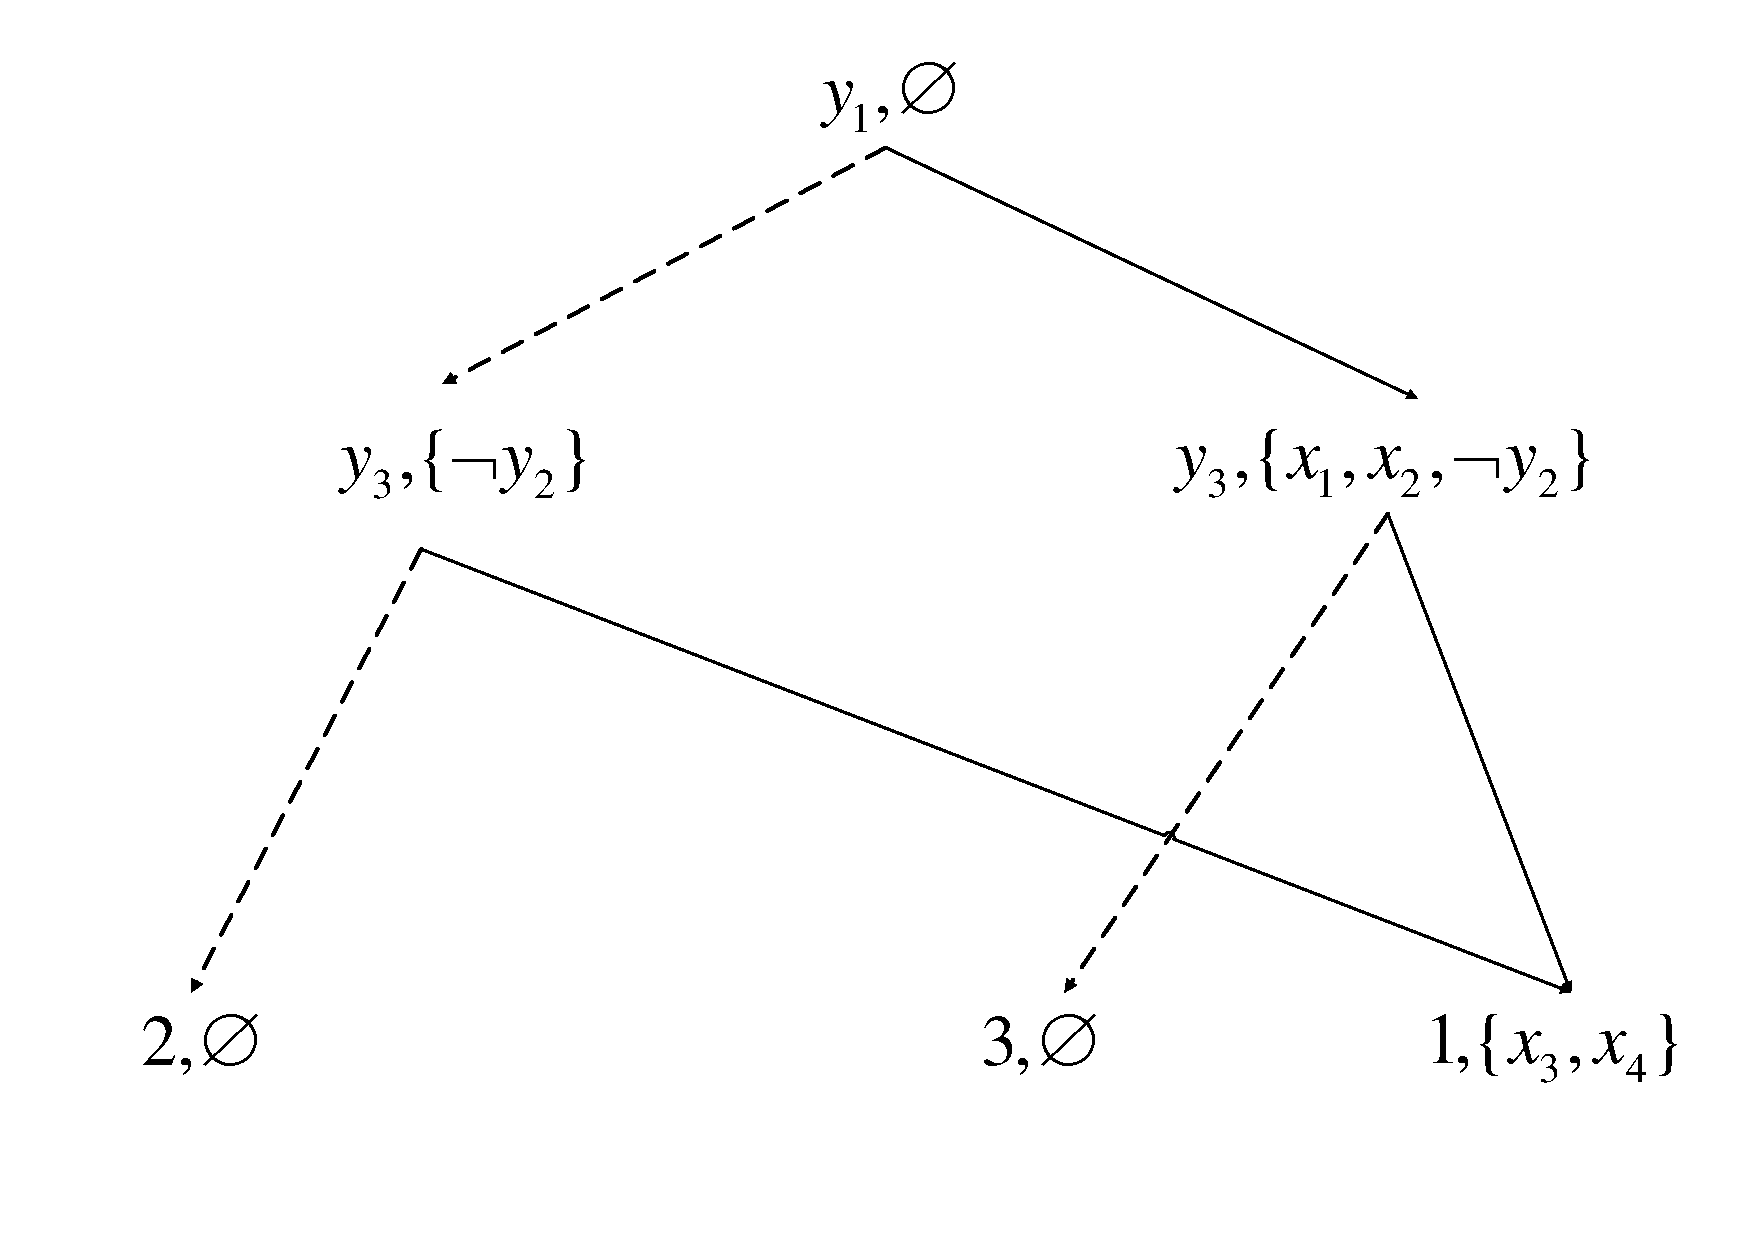
\includegraphics[width=0.7\linewidth]{figures/ADD-L-example2.pdf}
	\caption{An ADD-L example corresponding to Example \ref{circuit-example}, where the implied literals include the variables in $X$. }
	\label{fig:ADDL-example2}
\end{figure} 

\textbf{Implied Literal}
From the definition of entropy, the assignment $\sigma$ is restricted to $Y$, so the implied literals theoretically only contain variables from $Y$.
%However, we observed that if the implied literals are not restricted to only variables in $Y$ and can also include variables in $X$, it can further simplify the formula and optimize the structure of ADD-L.
However, we observed that the structure of ADD-L can be further simplified and optimized if the implied literals are not limited to variables in $Y$ but can also include variables in $X$.
Based on this observation, we made some improvements to the computation of implied literals, removing restrictions on implied literals to allow them to include variables in $X$. Additionally, we found that this technique can enhance the efficiency of the search without compromising the accuracy of entropy computation.
We use an example to illustrate the correctness and effectiveness of this idea, as shown in Figure \ref{fig:ADDL-example2}.
%It is easy to see from the comparison between Figure \ref{fig:ADDL-example2} and Figure \ref{fig:ADDL-example1} that this approach optimizes the structure of ADD-L without affecting the entropy result.
From the comparison between Figure \ref{fig:ADDL-example1} and \ref{fig:ADDL-example2}, it is easy to see that the approach optimizes the structure of ADD-L without affecting the entropy result.

\textbf{Variable Decision Heuristic} 
We apply the current state-of-the-art model counting heuristics to the Shannon entropy computing problem and perform experimental comparisons, including \textbf{VSADS}~\cite{sang2005heuristics}, \textbf{minfill}~\cite{darwiche2009modeling}, \textbf{SharpSAT-TD heuristic}~\cite{korhonen2021integrating}, and \textbf{DLCP}~\cite{lai2021power}.
We experimented with these heuristics, and our experiments show that the \textbf{minfill} heuristic is the one that performs best in the entropy computing problem. 
We use the \textbf{minfill} heuristic by default in our subsequent experiments.

\textbf{Preprocessing} 
%Since the core of entropy computing is model counting, we try to integrate the preprocessing strategy in model counting into our entropy tool PSE.
%Based on Literal Equivalences, which is a powerful technique in SAT solving, we implement a new preprocessing approach in PSE.
Since model counting is the core of entropy computing, we extend the preprocessing technique based on literal equivalence in model counting and integrate it into our entropy tool, PSE.
This idea is inspired by the work of Lai et al. \cite{lai2021power} on capturing literal equivalence in knowledge compilation.
However, due to the special nature of the entropy computing process, we cannot arbitrarily replace the literals corresponding to variables in the output set with equivalent ones.
%This is because the new formula $\varphi '$ obtained after the equivalent substitution of literals is equivalent to $\varphi$ in model counting, but not necessarily equivalent in entropy (it is not equivalent when the variables corresponding to the substituted literals belong to $Y$).
%At the beginning, we had a simple idea to restore all equivalent literals after the calculation, in order not to affect the calculation of the entropy and at the same time to reduce the size of the formula.
This is because the new formula $\varphi'$ obtained after the equivalent substitution of literals is equivalent to $\varphi$ in model counting, but not necessarily equivalent in entropy (it is not equivalent when the variables of substituted literals belong to $Y$).
In the beginning, we had the simple idea of restoring all equivalent literals after the calculation so as not to affect the calculation of the entropy and, at the same time, reduce the size of the formula.
We improve this idea by restoring only the literals corresponding to the variables in $Y$, since the assignments that affect the entropy are only in the part of $Y$. 
The new preprocessing method is called \textbf{Pre} in the following.
Experiments have demonstrated that this preprocessing method provides some performance enhancement to the tool (See Section \ref{sec:Experiments}).
This idea of preprocessing is motivated by the fact that, on the one hand, after preprocessing using literal equivalence, it can simplify the formula and thereby improve the efficiency of the subsequent model counting.
On the other hand (and more importantly), it reduces the treewidth of the tree decomposition, which leads to a more optimal order of variable selection obtained by the tree decomposition heuristic, and can be very effective in improving the efficiency of PSE calculations.




\begin{comment}
	Algorithm \ref{Condition} describes another model counting method in $X$-stage.
	To implement this method, a prerequisite is that we need an ADD-L constructed based on the original minfill static variable order. The difference between this ADD-L and the ADD-L corresponding to Algorithm 2 is that the $Y$-stage of Algorithm 2 is equivalent to making decisions only on the variables of the $Y$ set based on the minfill static variable order, while our new idea is to make decisions on all variables in the order of the minfill static variable order (including var in $X$). 
	The motivation for this is that our experiments have found that the heuristic effect of the minfill linear order is much stronger (making decisions only on the variables of the $Y$ set to some extent disrupts the linear order). 
	At this point, the computing process is more like general model counting, which can efficiently construct ADD-L. 
	With such an ADD-L, we can utilize conditional model counting (or entropy computing) in knowledge compilation to solve the model counting in the $X$-stage. 
	Lines 1-2 of the algorithm indicate that when the result of a node hits the cache, we can directly retrieve the corresponding result from the cache. 
	When accessing a terminal node, we directly return the result of the corresponding terminal node (lines 4-5). 
	If the variable decision of node u is false, we recursively call the lo branch to solve it (lines 7-8). 
	Similarly, when the variable decision of node u is true, we recursively call the hi branch to solve it (lines 10-11). Otherwise, it means that the variable corresponding to the node has not been decided, so both lo and hi need to be called (line 13). 
	We cache the current result and return it in lines 14-15.
	
	
	
	If any remaining variables in $Y$ have not been assigned values, we make decisions about them in lines 8-10.
	First, a variable x is chosen heuristically.
	Next the $infor$ of the subformula is computed recursively for two different values (true, false) of $x$. 
	Finally, the $infor$ of the two subformulas ($\varphi[y \mapsto false]$ and $\varphi[y \mapsto true]$) are summed to obtain the $infor$ of the current formula, and the $infor$ associated with the corresponding formula is added to the cache.
	
	Whenever we obtain a satisfiable assignment $\sigma_{\downarrow Y}$ under the restriction of the output set $Y$, we need to calculate the number of different inputs corresponding to this assignment.
	This step can be achieved by performing model counting on the remaining formulas (corresponding to the numerator of $p_{\sigma}$).
	According to \ref{projected-proposition},  the denominator of  $p_{\sigma}$ can be represented by the total number of models of $\varphi$, from which $p_{\sigma}$ can be calculated, and then the $infor$ of the sub-formula can be derived.
	Algorithm \ref{InforComputing} describes this process. 
	
	Algorithm \ref{InforComputing} receives a remaining CNF formula $\Phi$ after all variables in $Y$ have been assigned and returns the $infor$ $H(\varphi)$ of $\Phi$.
	As mentioned above, we perform model counting on the remaining sub-formulas in lines 1-4.
	In the model counting of the $X$-stage, we propose two methods, called \textbf{Counting} and \textbf{Condition}, with $count_{opt}$ as a parameter to indicate the chosen method.
	The first approach corresponds to lines 1-2, where any exact model counting tool can be called. 
	It's worth noting that this method does not just query the model counting individually.
	Instead, we share the component cache for all model counting queries, and we refer to this strategy as \textbf{XCache}.
	The other method requires constructing in advance an ADD-L that contains all the variables in $Y$, which can also include variables from the $X$.
	Then convert the model counting into conditional model~\cite{lai2017new} counting based on the current variable assignment.
	In line 5, probability $p_{\sigma}$ is computed according to the definition in Section 2, where $totalcount$ is the number of models of the entire formula $\varphi$, which is also computed by a model counting tool. 
	We only need to calculate $totalcount$ once and store it. 
	In line 6, the $infor$ can be obtained from $p_{\sigma}$ and returned as a result in line 7.
	
\end{comment}

